\documentclass[]{article}
\usepackage[
            left=1in,right=1in,top=1in,bottom=1in,%
            footskip=.25in]{geometry}
\usepackage{enumitem}
\usepackage{array}
\usepackage{amsmath}
\usepackage{amssymb}
\usepackage{graphicx}
\usepackage{verbatim}
\usepackage{hyperref}
\usepackage{subcaption}
\usepackage{float}
\usepackage{physics}
\usepackage{mwe}
\usepackage{graphicx}
\usepackage{pbox}
\usepackage{multicol}
\usepackage[utf8]{inputenc}
\hypersetup{
    colorlinks=true,
    linkcolor=blue,
    filecolor=magenta,      
    urlcolor=cyan,
}

\setlength{\arrayrulewidth}{0.2mm}
\setlength{\tabcolsep}{5pt}
\renewcommand{\arraystretch}{1.5}
\newcolumntype{L}{>{$}c<{$}}


%opening
\title{Causal Inference with Complex Dynamical Systems}
\author{George Stepaniants}

\begin{document}

\maketitle
\begin{abstract}
Causal inference is a large and long-standing field that attempts to answer a very fundamental question: does X cause Y? This question arises in many fields such as healthcare, genomics, biology, and econometrics. The complex systems analyzed in these fields often have many interacting components mathematically represented as nodes and edges (connectivity) of a network. Network inference is the study of the time-dependent behavior of these nodes to reverse-engineer the network connectivity. The theory of causal inference has many contending definitions of causality such as state-of-the-art techniques Granger Causality (GC) and Convergent Cross Mapping (CCM). These algorithms are computationally tractable and easy to use but require strong mathematical assumptions. We simulate networks of harmonic and Kuramoto oscillators and attempt to reconstruct their ground-truth network structure using observations of oscillator displacements over time. Our analysis investigates the performance of inference methods on Erdos-Renyi and scale-free random graphs. We show that the GC and CCM inference methods systematically fail to determine network structure by returning overly sparse or dense connectivity results. These findings challenge the applications of such top-down inference approaches to physical and biological systems. Using a few basic assumptions, we demonstrate how networked systems of coupled oscillators can be successfully reconstructed if perturbations of the system are allowed. We propose a Perturbation Causal Inference (PCI) algorithm that uses systematic perturbations and tracks how perturbation cascades spread through the network. Using changepoint detection, correlation, and windowed variance statistics, we predict causal relationships between nodes in the graph. Our analysis shows that PCI works at scale and efficiently returns high accuracy reconstructions of large networks with varying coupling strengths and connectivity structures. We conclude by proposing future applications of perturbation inference methods into neuroscience and make a connection with Hebbian learning rules.
\end{abstract}

\section{Introduction and Overview}
Since the birth of the scientific method, we have learned how to formulate a question and test a hypothesis through the use of an experimental study. In causal inference, the question we ask is ?does X cause Y?? The earliest attempts to solve this question can be traced to the philosophical debates of ? The first scientific approach to causal inference was through the use of controlled experiments. In a controlled experiment, given a system S, a parameter X, and a measurement Y = m(S) an intervention is performed to change X while keeping all other parameters fixed. This determines whether changing X causes a significant change in Y (i.e. if there is a causal effect). This approach has led to many fundamental discoveries in experimental physics and biology [cite lab experiments]. However, even for a controlled experiment in a laboratory setting it is often impossible to fix all the important parameters of a system. 

This problem becomes even harder when inferring causal relationships in the real world such as patient studies, population dynamics, and social media because of the random fluctuations within samples. One of the earliest studies of causality came from the work of Jerzy Neyman who laid down the framework of potential outcomes and randomized experiments in his 1923 Master?s thesis on agricultural experimentation [cite Neyman?s thesis]. In this context, ?individuals? are randomly assigned to varying levels of treatment and each individual has a different potential outcome for each treatment value. Since each individual can only be assigned one treatment, we cannot observe what the outcome for the same individual would be in a different treatment group (i.e. we cannot observe their alternative futures). This is called the ?fundamental problem of causal inference? from which it naturally follows that causality cannot be deduced at the individual level. Neyman showed how the average of the individual level causal effect can be estimated in a fully randomized experiment by randomly assigning individuals to different treatment groups and taking the different between the expected outcome in treatment and control. This framework was then extended by Donald Rubin 

C.W. Granger stated that ?causality is a concept whose definition people know what they do not like but few know what they do like? [cite Granger?s personal note].

Norbert Weiner first defined it in his paper by saying that X causes Y if knowing the past of X predicts Y?s future [cite Weiner?s book]. Granger further formalized this idea by phrasing it through vector autoregressive models (i.e. the simplest time-lagged linear models) [cite Granger?s personal note and original paper]. This definition of causality came to be known as ?Granger Causality? and gained sufficient popularity in the applied economics community because of its clear mathematical assumptions and ease of use [cite economics papers using GC]. Many fields including healthcare, genomics, biology, and econometrics attempt to find causal relationships between components of large systems in order to understand how behavior of one component influences the behavior of the rest. Examples commonly include large neuronal circuits, gene expression networks, and the stock market. Each component of the system can naturally be represented as a node of a directed network where each directed edge from node A to node B defines a causal relationship from A to B (i.e. an increase in the price of stock A causes an increase in the price of stock B). By its original definition, Granger causality **(talk about pairwise GC)**. A number of research results show the success of Granger causality in inferring causal relationships in studies of such complex networked systems [cite econ and neuroscience GC papers]. 

Since the release of Granger?s seminal paper [cite GC here], many results have appeared showing the success of this method outside of economics in fields such as neurobiology and genetics. [cite bad GC application papers here]. However, these results rarely compare their inference

In the first part of this paper we evaluate the performance of Granger causality on physical systems where the ground-truth connectivity is known. We show that GC fails to recover the causal connections in networks of coupled harmonic and Kuramoto oscillators. We encourage the reader to study the theoretical assumptions of GC before applying it to data in physical and biological systems where those conditions may not be met.

Several research studies have highlighted that Granger causality does not imply real causality and does not satisfy our intuition behind causal relationships [cite papers that show evidence against GC including Bethany?s paper]. Granger himself stated in his personal note that ?causality is a concept whose definition people know what they do not like but few know what they do like? [cite Granger?s personal note].
\section{Causal Inference Methods}
\subsection{Granger Causality}

\subsection{Convergent Cross Mapping}

\subsection{Perturbation Inference}


\section{Oscillator Systems}
\subsection{Harmonic Oscillators}
The standard equation for the displacement $x$ of a damped harmonic oscillator with mass $m$, spring constant $k$, and damping constant $c$ is
\begin{align*}
m\frac{d^2x}{dt^2} = -kx - c\frac{dx}{dt}
\end{align*}

The system we investigate in this paper is $n$ coupled harmonic oscillators where $\mathbf{x}$ is the vector of displacements of all oscillators in the system and $\mathbf{m}$ is the vector of their masses. This network of oscillators has fixed boundary conditions so the 1st and nth oscillators are attached to fixed walls by springs. Also, pairs of oscillators in the network are connected to each other by springs with varying spring constants. A picture of a possible network configuration is shown in Figure [?].

\begin{figure}
    \centering
    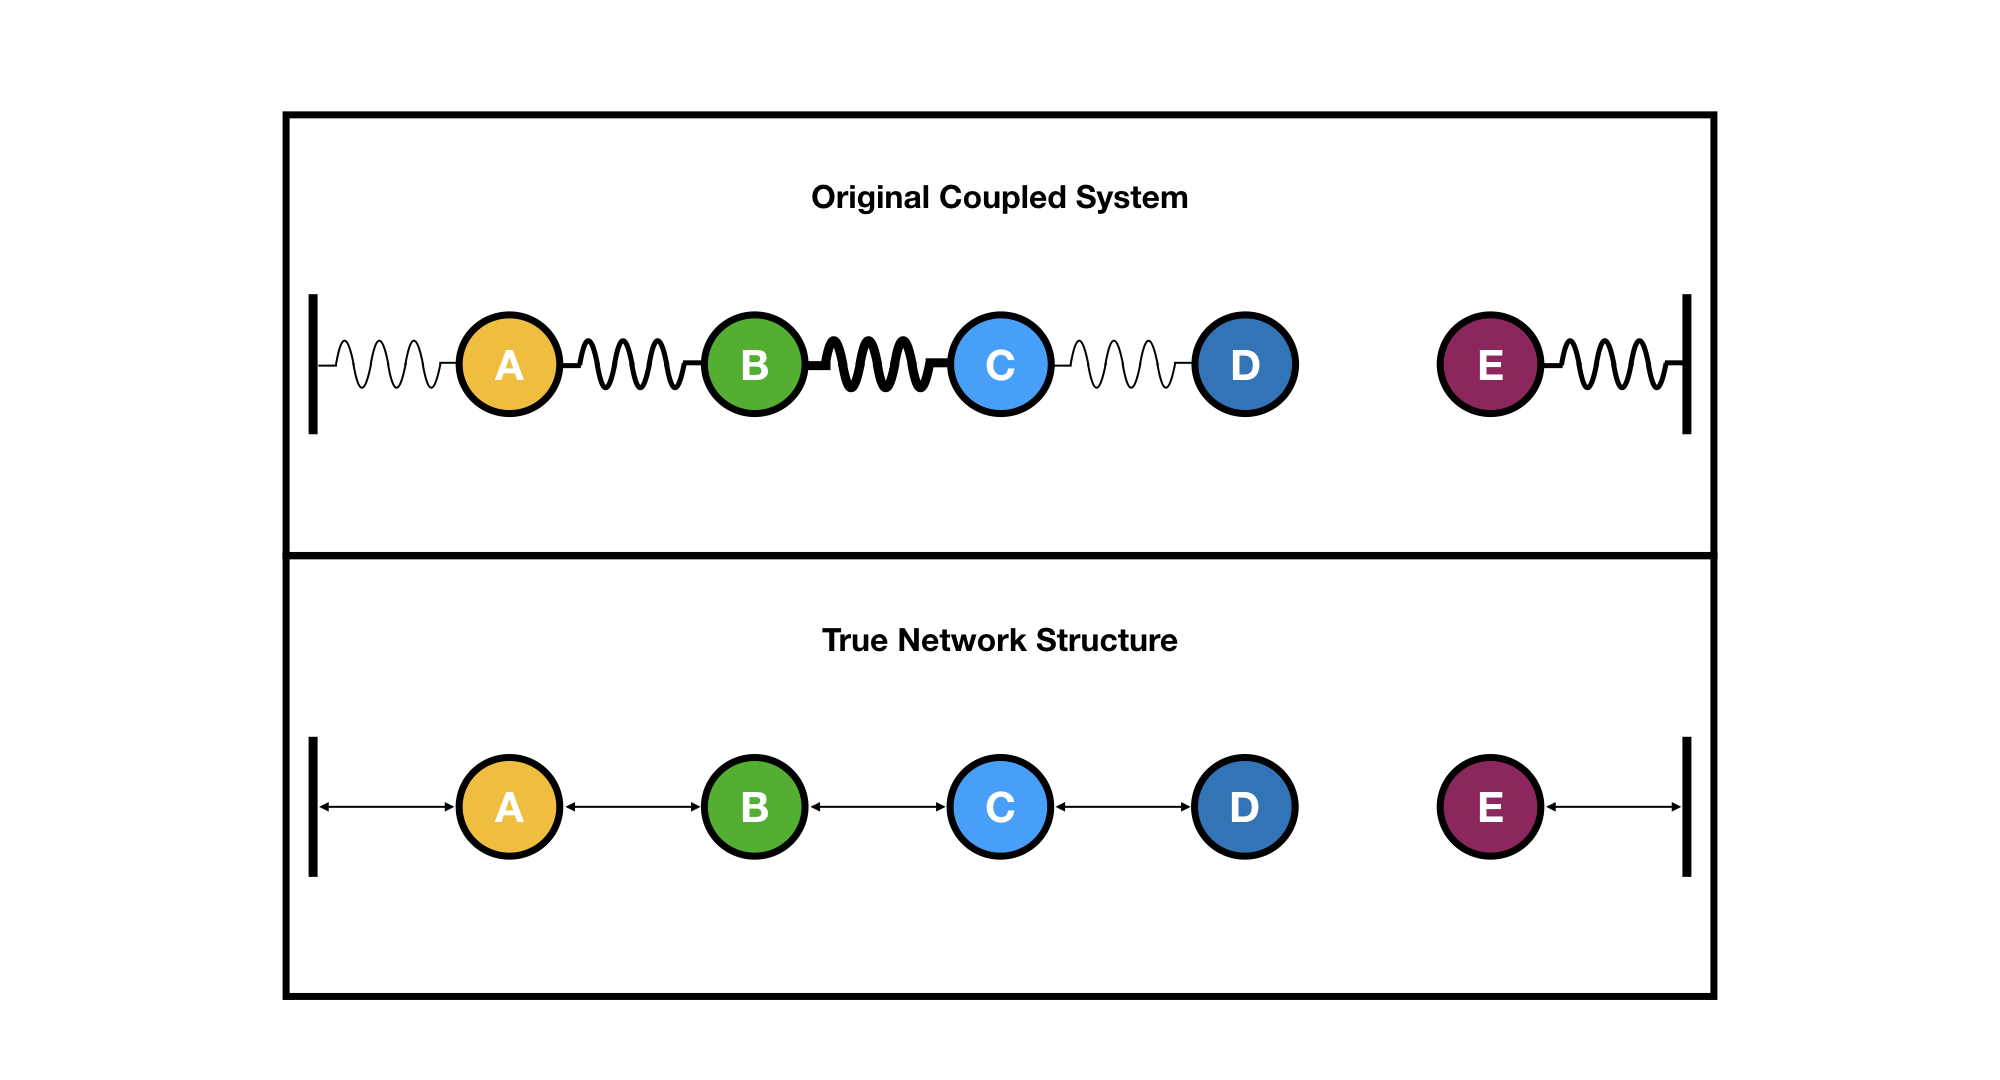
\includegraphics[width=14cm]{ExampleNetwork.jpeg}
    \caption{Example network of 5 harmonic oscillators with fixed boundary conditions and symmetric interactions.}
    \label{fig:example}
\end{figure}

Strength of coupling between oscillators and walls in this network is denoted by the $n + 1 \times n + 1$ matrix of spring constants $A$. The spring constant from oscillator $i$ to oscillator $j$ is denoted by $A_{ji}$. Note that in a physical system of harmonic oscillators, the coupled interactions between pairs of oscillators are symmetric so $A_{ij} = A_{ji}$ for all $1 \leq i, j \leq n$.

The system of ODEs that governs the movement of these oscillators is
\begin{align*}
\mathbf{m} \circ \frac{d^2\mathbf{x}}{dt^2} = A\mathbf{x} - c\frac{d\mathbf{x}}{dt}
\end{align*}
where $\circ$ is the element-wise or Hadamard product. Figure [?] shows the trajectories of a system of 3 coupled harmonic oscillators.

\subsection{Directed Harmonic Oscillators}
Causality by its nature is a directed relationship where $i$ causes $j$. However, causality is not necessarily symmetric and it is quite possible that $j$ doesn't cause $i$. As an example, rainy weather might cause more people to wear umbrellas but certainly umbrellas do not cause it to rain. Therefore, we are interested in finding how to infer asymmetric or directional causal relationships. In order to test the causal inference methods described in Section 2, we extend our model of coupled harmonic oscillators to have directed interactions between oscillators. Therefore, in equation [?] we relax the symmetry constraint on matrix $A$ so that the coupling strengths $A_{ij}$ and $A_{ji}$ can be different.

Doing so introduces two scenarios in which the solutions to this equation are poorly behaved. If at least one of the eigenvalues of the system are nonnegative, the solution to [?] will not converge. Section 7.1 in Appendix A describes how to compute the eigenvalues of this system **update this section**. From this section onwards, in our simulations of directed harmonic oscillators we only use coupling matrices $A$ such that the eigenvalues of [?] are negative.  Figure [?] shows a possible network configuration with asymmetric interactions between nodes.

\begin{figure}[H]
    \centering
    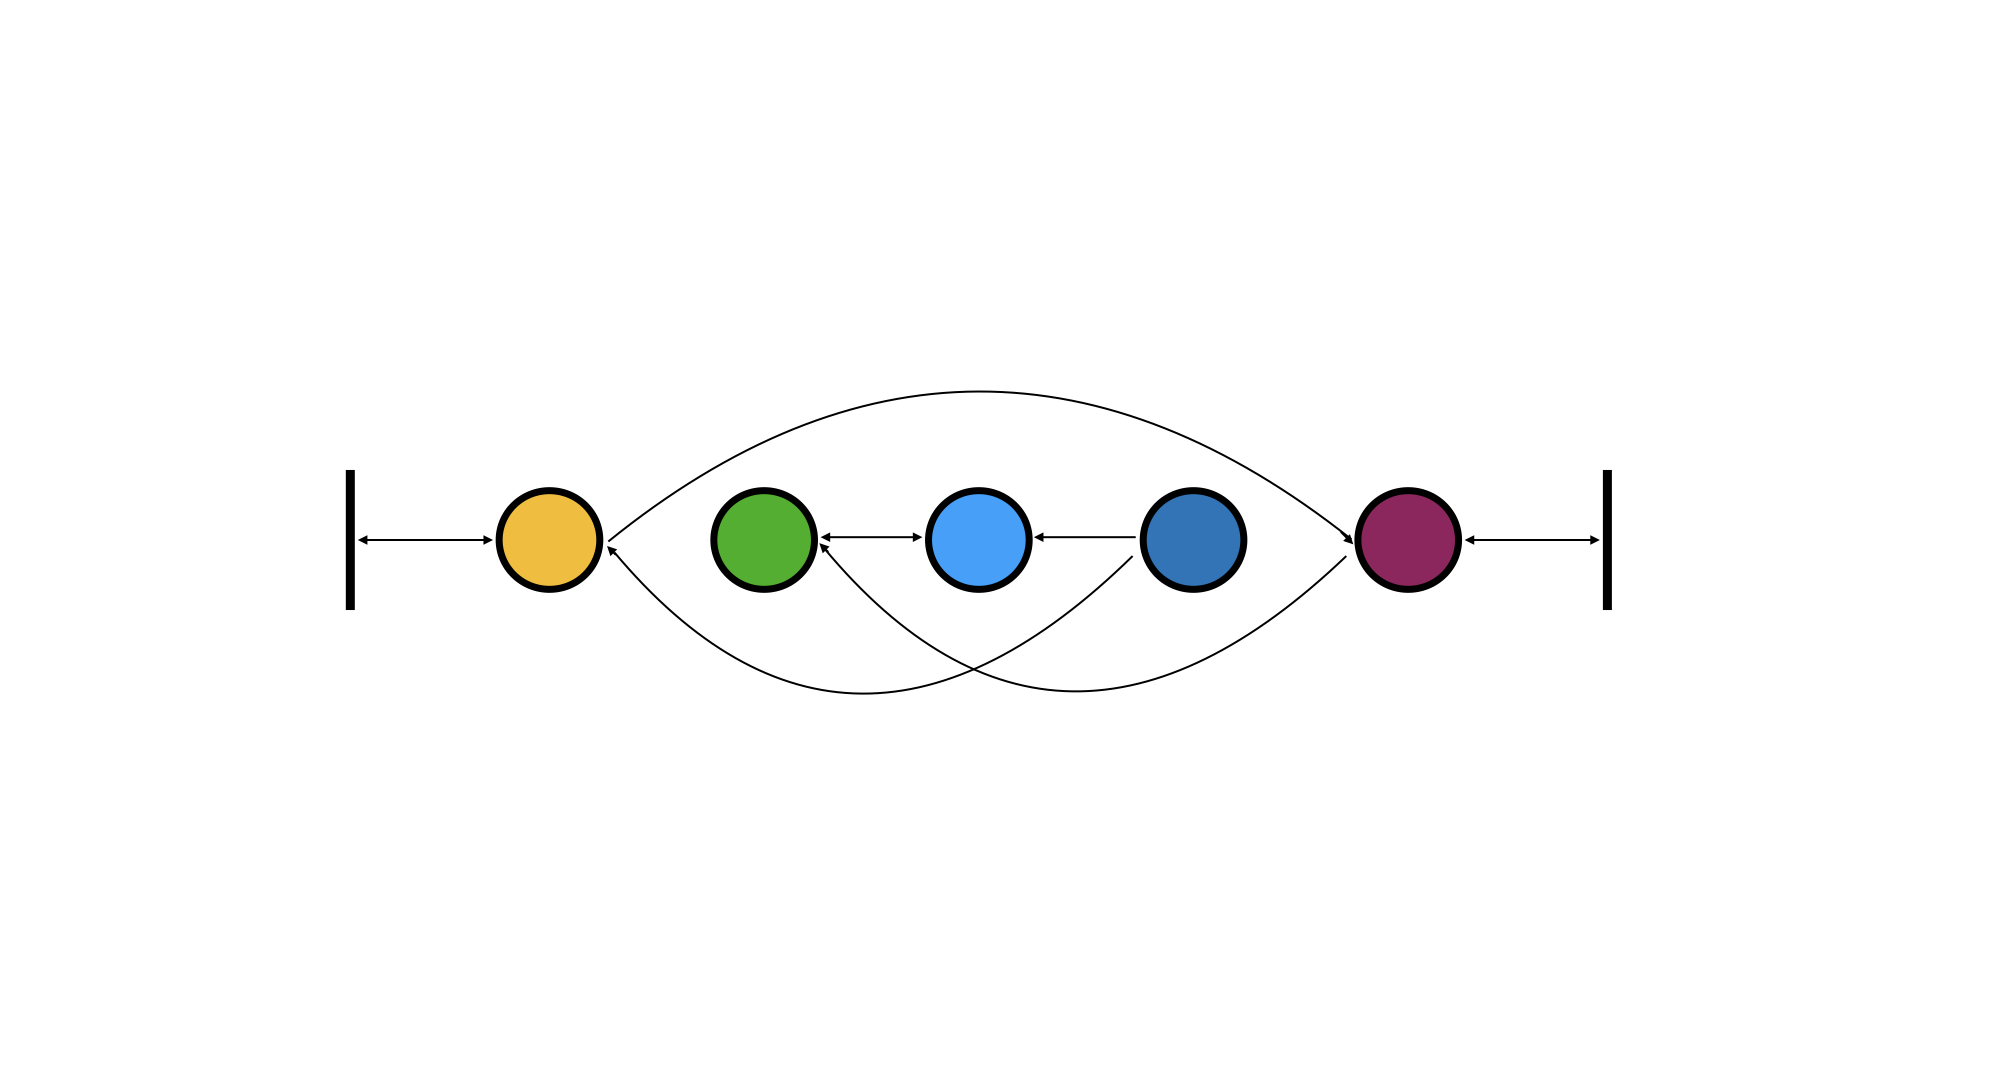
\includegraphics[width=14cm]{AsymmetricExampleNetwork.jpeg}
    \caption{Example network of 5 harmonic oscillators with fixed boundary conditions and asymmetric interactions.}
    \label{fig:example}
\end{figure}


\subsection{Kuramoto Oscillators}



\section{Numerical Experiments}
Used MVGC toolbox for GC. Used rEDM toolbox for CCM.


\renewcommand{\thesubsection}{\Alph{subsection}}
\section{Computational Results}
\subsection{Inference for Two Oscillator System}
Here we investigate the ability of GC and CCM to infer the structure of a two-node network. We evaluate these inference algorithms over all 4 possible two-node networks while varying the connection strengths in the system from 0.1 to 10 collectively. Figure 1 shows the confusion matrix for GC inference over all possible directed networks of two harmonic and Kuramoto oscillators. As we can see, GC makes strongly biased predictions that two oscillator networks are fully connected. The results of CCM inference on the same dataset of all possible two-node harmonic and Kuramoto oscillator networks are shown in Figure 2. CCM has a tendency to underestimate or overestimate the number of connections in these two-node networks and performs poorly on networks with one directed edge.


\subsection{Inference on Erdos-Renyi Networks}
In the next experiments, we evaluate GC and CCM on random Erdos-Renyi networks with 3 or more nodes. Every edge in an Erdos-Renyi network has a probability $p$ that it exists. We generate 20 Erdos-Renyi networks by varying $p$ from 0.05 to 1 and also vary the collective connection strengths from 0.1 to 10.

Figures 3, 4, and 5 show the performance of GC and CCM on these random networks for 3, 4, and 5 nodes respectively.


\subsection{Perturbation Inference for Two Oscillator System}
Figure 3 shows the confusion matrix for PC inference over all possible directed networks of two harmonic or Kuramoto oscillators with one node perturbed.

Figure 4 shows the confusion matrix for PC inference over all possible directed networks of two harmonic or Kuramoto oscillators with both nodes perturbed.

The performance of PC is shown for different combinations of network connection probabilities and spring constants in Figure 5.

\begin{figure}
    \centering
    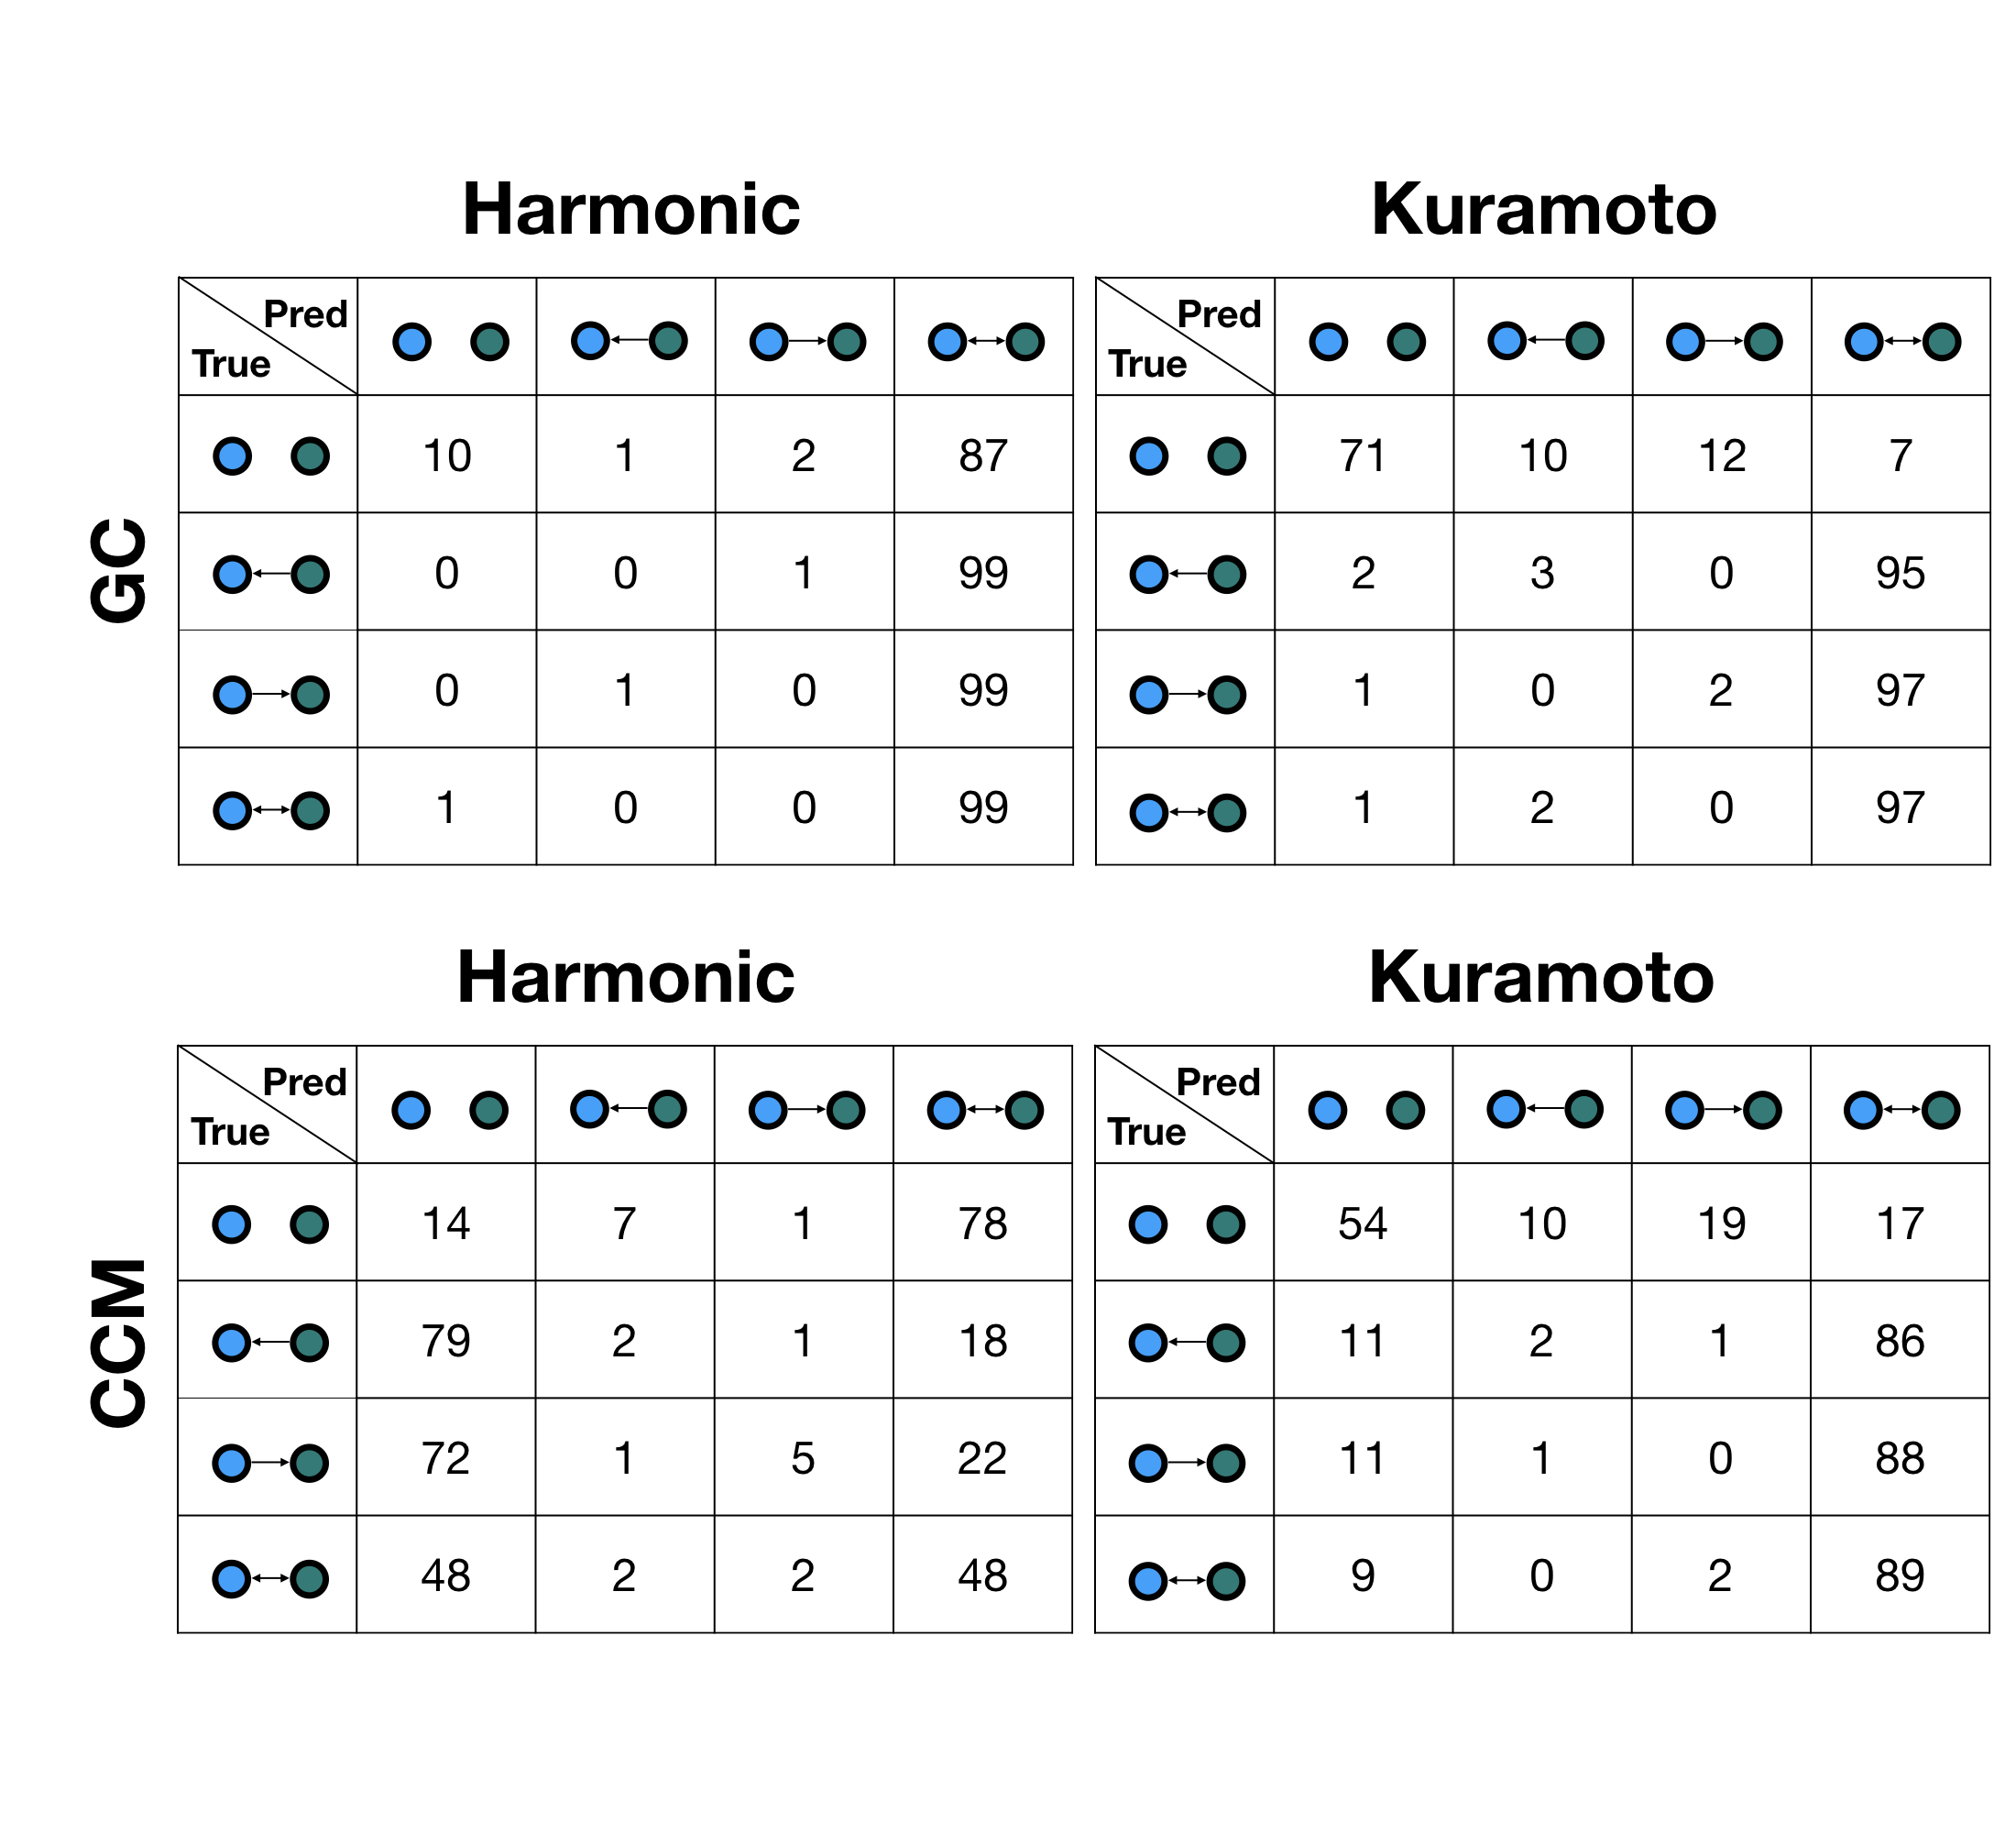
\includegraphics[width=12cm]{TwoNodeConfusionMatrix.jpeg}
    \caption{Confusion matrix for GC and CCM on networks of two oscillators.}
    \label{fig:example}
\end{figure}

\begin{figure}
    \centering
    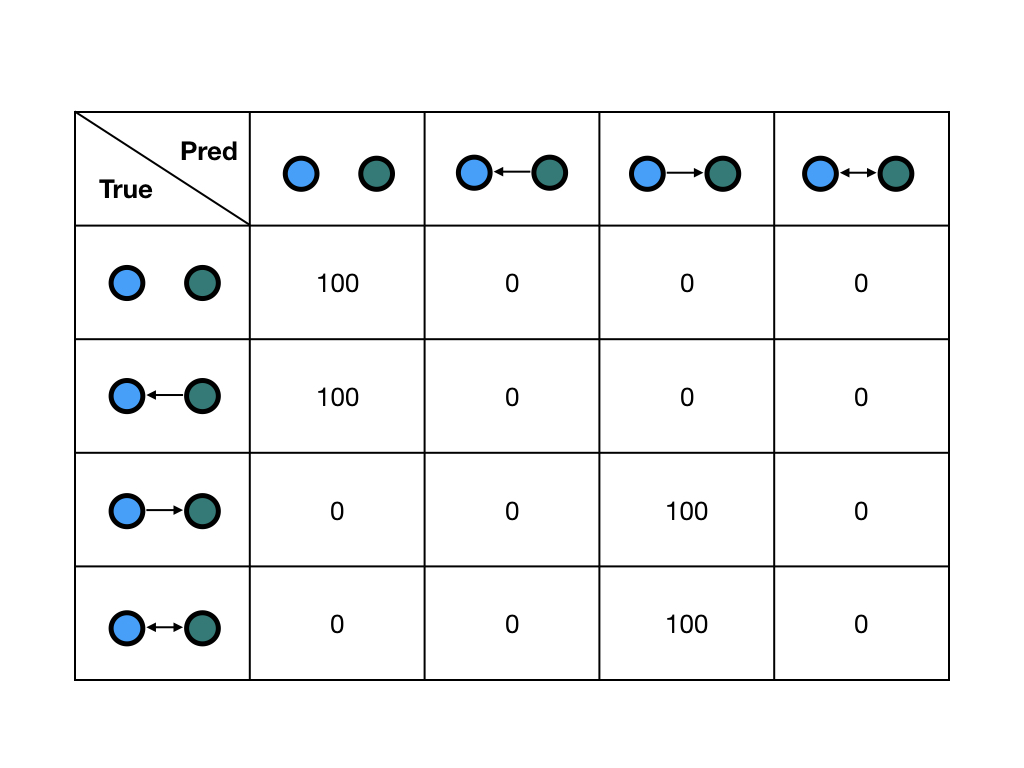
\includegraphics[width=12cm]{Pert1ConfusionMatrix.jpeg}
    \caption{Confusion matrix for PC on networks of two oscillators with all nodes observed and only blue node perturbed.}
    \label{fig:example}
\end{figure}

\begin{figure}
    \centering
    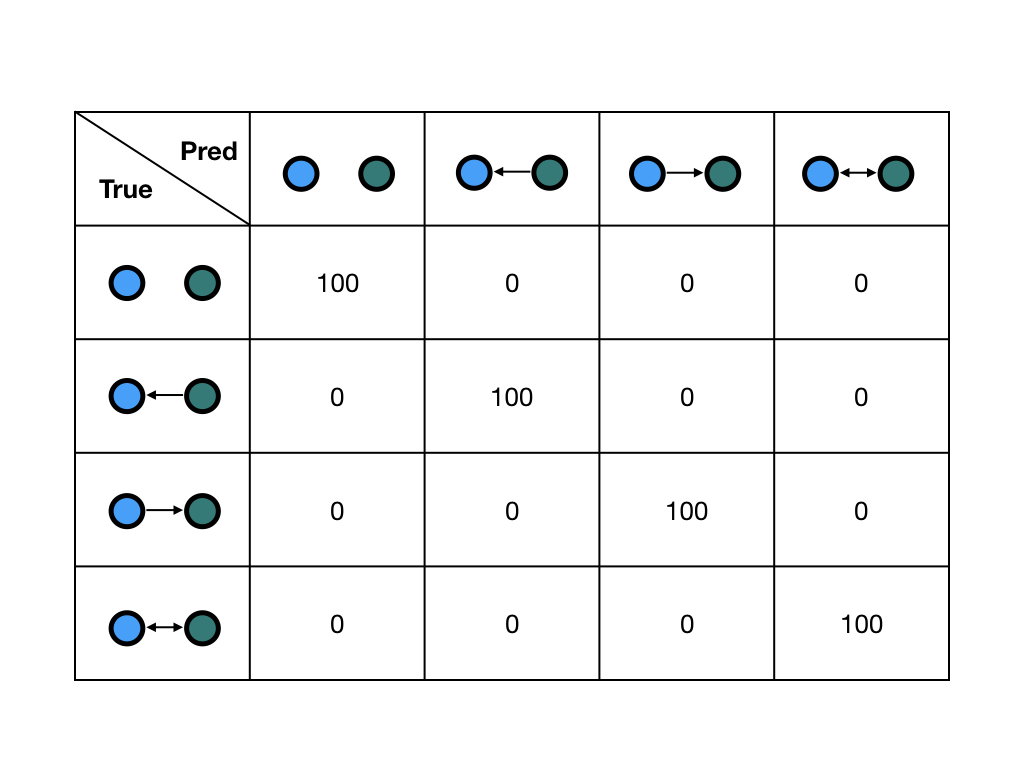
\includegraphics[width=12cm]{Pert2ConfusionMatrix.jpeg}
    \caption{Confusion matrix for PC on networks of two oscillators with all nodes observed and perturbed.}
    \label{fig:example}
\end{figure}

\begin{figure}
    \centering
    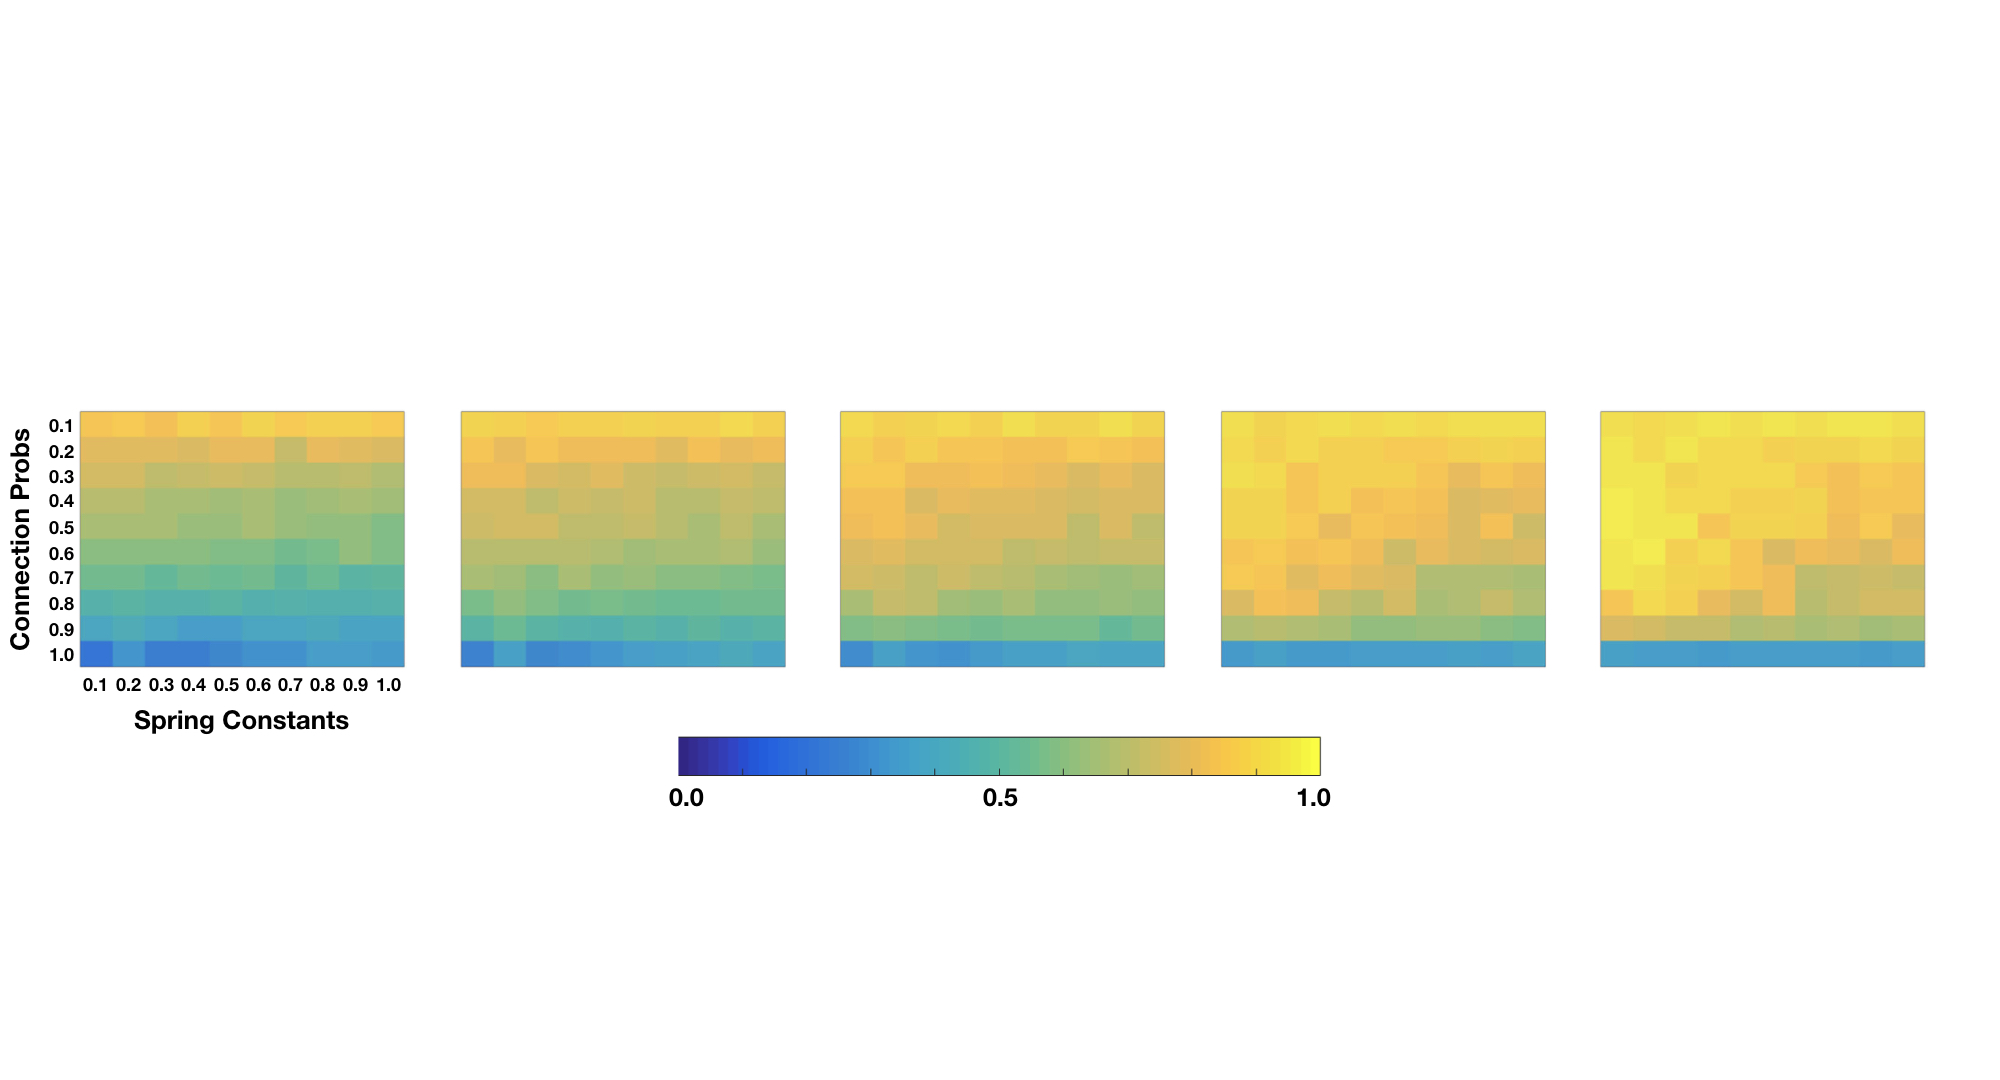
\includegraphics[width=15cm]{VaryStrengthsProbs.jpeg}
    \caption{Accuracy of PC over varying network connections probabilities and spring constants. All nodes can be observed and each matrix shows the results when 2, 4, 6, 8, and 10 nodes are perturbed respectively.}
    \label{fig:example}
\end{figure}

\subsection{Inference for N Oscillators}
Give statistics like accuracy, TPR, FPR over different simulations of N oscillators. Don't damp or do anything special with the simulation parameters.

\subsection{Inference with Damped Oscillator System}
Give statistics like accuracy, TPR, FPR over different simulations of N oscillators.


\section{Analysis}
\subsection{Reasons why Granger Causality works with Perturbed Harmonic Oscillator Data}


% Tables for all experiments
\clearpage
\begin{table}
\tiny
\begin{tabular}{| c | L | c | L | L | L | L | L | c | L | L | L | L | c | L |}
\hline
\multicolumn{15}{|c|}{Summary of GC Experiments for Harmonic Oscillators} \\
\hline
\hline
\textbf{Experiment Name} & \mathbf{n} & $\mathbf{A}$ & \mathbf{K} & \mathbf{m} & \mathbf{p_0} & \mathbf{v_0} & \mathbf{\gamma} & \textbf{Forcing} & \mathbf{N} & \mathbf{\Delta t} & \mathbf{T} & \mathbf{s} & \textbf{Prep} & \textbf{Reps} \\
\hline
gcH1 & 2 & All four two-node networks & 0.1, 0.2, ..., 10 & 1 & [-0.5, 0.5] & 0 & 0 & None & 100 & 0.1 & 25 & 0.1 & Detrend & 1 \\
\hline
gcH5 (deviate with small mass) & 5 & ER $p=0.5$ & 1 & ^a & ^b & 0 & 0 & None & 100 & 0.1 & 25 & 0.1 & Detrend & 1 \\
\hline
gcH6 (deviate with large damping, show diff K) & 5 & ER $p=0.5$ & 0.1, 0.2, ..., 10 & 1 & ^b & 0 & 10 & None & 100 & 0.1 & 25 & 0.1 & Detrend & 1 \\
\hline
\end{tabular}
\\[1cm]


\begin{tabular}{| c | L | c | L | L | L | L | c | L | L | L | L | c | L |}
\hline
\multicolumn{14}{|c|}{Summary of GC Experiments for Kuramoto Oscillators} \\
\hline
\hline
\textbf{Experiment Name} & \mathbf{n} & $\mathbf{A}$ & \mathbf{K} & \mathbf{\theta_0} & \mathbf{\omega} & \mathbf{\gamma} & \textbf{Forcing} & \mathbf{N} & \mathbf{\Delta t} & \mathbf{T} & \mathbf{s} & \textbf{Prep} & \textbf{Reps} \\
\hline
gcK1 & 2 & All four two-node networks & 0.1, 0.2, ..., 10 & [0, 2\pi] & [-1, 1] & 0 & None & 100 & 0.1 & 25 & 0.1 & Detrend & 1 \\
\hline
gcH6 (deviate with large damping, show diff K) & 5 & ER $p=0.5$ & 0.1, 0.2, ..., 10 & [0, 2\pi] & [-1, 1] & 10 & None & 100 & 0.1 & 25 & 0.1 & Detrend & 1 \\
\hline
\end{tabular}
\\[1cm]


\begin{tabular}{| c | L | c | L | L | L | L | L | c | L | L | L | L | c | L |}
\hline
\multicolumn{15}{|c|}{Summary of CCM Experiments for Harmonic Oscillators} \\
\hline
\hline
\textbf{Experiment Name} & \mathbf{n} & $\mathbf{A}$ & \mathbf{K} & \mathbf{m} & \mathbf{p_0} & \mathbf{v_0} & \mathbf{\gamma} & \textbf{Forcing} & \mathbf{N} & \mathbf{\Delta t} & \mathbf{T} & \mathbf{s} & \textbf{Prep} & \textbf{Reps} \\
\hline
ccmH1 & 2 & All four two-node networks & 0.1, 0.2, ..., 10 & 1 & [-0.5, 0.5] & 0 & 0 & None & 100 & 0.1 & 25 & 0.1 & Detrend & 1 \\
\hline
ccmH5 (deviate with small mass) & 5 & ER $p=0.5$ & 1 & ^a & ^b & 0 & 0 & None & 100 & 0.1 & 25 & 0.1 & Detrend & 1 \\
\hline
ccmH6 (deviate with large damping, show diff K) & 5 & ER $p=0.5$ & 0.1, 0.2, ..., 10 & 1 & ^b & 0 & 10 & None & 100 & 0.1 & 25 & 0.1 & Detrend & 1 \\
\hline
\end{tabular}
\\[1cm]


\begin{tabular}{| c | L | c | L | L | L | L | c | L | L | L | L | c | L |}
\hline
\multicolumn{14}{|c|}{Summary of CCM Experiments for Kuramoto Oscillators} \\
\hline
\hline
\textbf{Experiment Name} & \mathbf{n} & $\mathbf{A}$ & \mathbf{K} & \mathbf{\theta_0} & \mathbf{\omega} & \mathbf{\gamma} & \textbf{Forcing} & \mathbf{N} & \mathbf{\Delta t} & \mathbf{T} & \mathbf{s} & \textbf{Prep} & \textbf{Reps} \\
\hline
ccmK1 & 2 & All four two-node networks & 0.1, 0.2, ..., 10 & [0, 2\pi] & [-1, 1] & 0 & None & 100 & 0.1 & 25 & 0.1 & Detrend & 1 \\
\hline
ccmH6 (deviate with large damping, show diff K) & 5 & ER $p=0.5$ & 0.1, 0.2, ..., 10 & [0, 2\pi] & [-1, 1] & 10 & None & 100 & 0.1 & 25 & 0.1 & Detrend & 1 \\
\hline
\end{tabular}
\\[1cm]


\begin{tabular}{| c | L | L | L | c | L | L | L | L | L | c | L | L | L | L | c |}
\hline
\multicolumn{14}{|c|}{Summary of PC Experiments for Harmonic Oscillators} \\
\hline
\hline
\textbf{Experiment Name} & \mathbf{n} & \mathbf{n_\text{pert}} & \mathbf{n_\text{obs}} & $\mathbf{A}$ & \mathbf{K} & \mathbf{m} & \mathbf{p_0} & \mathbf{v_0} & \mathbf{\gamma} & \textbf{Forcing} & \mathbf{N} & \mathbf{\Delta t} & \mathbf{T} & \mathbf{s} & \textbf{Method} \\
\hline
pcH1 & 2 & 1, 2 & 1, 2 & All four two-node networks & 0.1, 0.2, ..., 10 & 1 & [-0.5, 0.5] & [-1, 1] & 0.1 & None & 100 & 0.1 & 25 & 0.1 & corr \\
\hline
pcH1 & 2 & 1, 2 & 1, 2 & All four two-node networks & 0.1, 0.2, ..., 10 & 1 & [-0.5, 0.5] & [-1, 1] & 0.1 & None & 100 & 0.1 & 25 & 0.1 & chngpt \\
\hline
pcH10 & 10 & 1, 2, ..., 10 & 10 & ER $p=0.1, 0.2, ..., 1$ & 1 & 1 & [-0.5, 0.5] & [-1, 1] & 0.3 & Pulse$^b$ & 10 & 0.1 & ^c & 0.1 & corr \\
\hline
pcH20 & 20 & 1, 2, ..., 20 & 1, 2, ..., 20 & ER $p=0.5$ & 0.1 & 1 & [-0.5, 0.5] & [-1, 1] & 0.3 & Pulse$^b$ & 10 & 0.1 & ^c & 0.1 & corr \\
\hline
pcH21 & 20 & 1, 2, ..., 20 & 1, 2, ..., 20 & BA $m=10$ & 0.1 & 1 & [-0.5, 0.5] & [-1, 1] & 0.3 & Pulse$^b$ & 10 & 0.1 & ^c & 0.1 & corr \\
\hline
\end{tabular}
\\[1cm]


\begin{tabular}{| c | L | L | L | c | L | L | L | L | c | L | L | L | L | c |}
\hline
\multicolumn{15}{|c|}{Summary of PC Experiments for Kuramoto Oscillators} \\
\hline
\hline
\textbf{Experiment Name} & \mathbf{n} & \mathbf{n_\text{pert}} & \mathbf{n_\text{obs}} & $\mathbf{A}$ & \mathbf{K} & \mathbf{\theta_0} & \mathbf{\omega} & \mathbf{\gamma} & \textbf{Forcing} & \mathbf{N} & \mathbf{\Delta t} & \mathbf{T} & \mathbf{s} & \textbf{Method} \\
\hline
pcK1 & 2 & 1, 2 & 1, 2 & All four two-node networks & 0.1, 0.2, ..., 10 & [0, 2\pi] & [-1, 1] & 0 & None & 100 & 0.1 & 25 & 0.1 & meanvar \\
\hline
pcK1 & 2 & 1, 2 & 1, 2 & All four two-node networks & 0.1, 0.2, ..., 10 & [0, 2\pi] & [-1, 1] & 0 & None & 100 & 0.1 & 25 & 0.1 & chngpt \\
\hline
pcK20 & 20 & 1, 2, ..., 20 & 1, 2, ..., 20 & ER $p=0.5$ & 0.1 & [0, 2\pi] & [-1, 1] & 0 & Pulse$^b$ & 10 & 0.1 & ^c & 0.1 & meanvar \\
\hline
pcK21 & 20 & 1, 2, ..., 20 & 1, 2, ..., 20 & BA $m=10$ & 0.1 & [0, 2\pi] & [-1, 1] & 0 & Pulse$^b$ & 10 & 0.1 & ^c & 0.1 & meanvar \\
\hline
\end{tabular}\\

\footnotesize{
$^a$ Make one mass very small compared to the rest\\
$^b$ Displace only one mass from equilibrium\\
$^b$ Short pulses of force for each perturbation\\
$^c$ $T$ changes in size to fit all perturbations in simulation
}
\end{table}


\clearpage
\section{Appendix A}
\subsection{Calculating Wait Time for Damped Harmonic Oscillators}
Our perturbation approach requires that the forcing perturbation in the oscillator system decays to zero before the next forcing perturbation can be applied. This requires that we calculate a wait time between perturbations for every simulation. Below we discuss how this wait time is computed for the case of coupled harmonic oscillators. The general equation for a harmonic oscillator network is
\begin{align*}
\frac{d^2\mathbf{x}}{dt^2} + c\frac{d\mathbf{x}}{dt} - M\mathbf{x} = \mathbf{F}(t)
\end{align*}
where the displacements $\mathbf{x}$ and forcing function $\mathbf{F}$ are vectors of length $n$. In our simulations, we make our forcing function be a step function of the form
\begin{align*}
\mathbf{F}(t) = \begin{array}{cc}
  \Big\{ & 
    \begin{array}{cc}
      \mathbf{0} & t < t_0 \\
      \mathbf{f}  & t_0 \leq t \leq t_0 + \Delta t \\
      \mathbf{0} & t > t_0 + \Delta t
    \end{array}
\end{array}
\end{align*}
where $t_0$ is the time of the perturbation and $\Delta t$ is the length of time under which the system is forced.

To solve this equation, let's first solve the homogeneous equation
\begin{align*}
\frac{d^2\mathbf{x}}{dt^2} + c\frac{d\mathbf{x}}{dt} - M\mathbf{x} = 0
\end{align*}
This equation has $n$ linearly independent solutions of the form $\mathbf{x}_i(t) = \mathbf{v}_ie^{\omega_i t}$ for $1 \leq i \leq n$. Substituting $\mathbf{x}_i$ into the homogeneous equation we have
\begin{align*}
(\omega_i^2 + c\omega_i - M)\mathbf{v}_i = 0
\end{align*}

This implies that $M\mathbf{v}_i = (\omega_i^2 + c\omega_i)\mathbf{v_i}$ so $\mathbf{v}_i$ is an eigenvector of $M$ with eigenvalue $\lambda_i = \omega_i^2 + c\omega_i$. Solving the quadratic equation for $\omega_i$, we have that
\begin{align*}
\omega_i = \frac{-c \pm \sqrt{c^2 + 4\lambda_i}}{2}
\end{align*}

Now note that if $w_i$ has a positive real part, then our solution to this differential equation will diverge. This agrees with experimental simulations. !!!Not sure how to deal with $\pm$ in quadratic equation solution so just taking plus here!!!

Now let's assume that $\Re(w_i) < 0$ for all $1 \leq i \leq n$. Using our forcing function $\mathbf{F}(t)$ defined above, let's solve our differential equation in the time $t \in [t_0, t_0 + \Delta t]$. In this time interval, $\mathbf{F}(t) = \mathbf{f}$ for some constant $f \in \mathbb{R}^n$ so
\begin{align*}
\frac{d^2\mathbf{x}}{dt^2} + c\frac{d\mathbf{x}}{dt} - M\mathbf{x} = \mathbf{f}
\end{align*}

If $\mathbf{x}_{hom}$ is the homogeneous solution to the equation above, then as long as the matrix $M$ is invertible, the general solution to our ODE is
\begin{align*}
\mathbf{x} = \mathbf{x}_{hom} - M^{-1}\mathbf{f}
\end{align*}

This indeed agrees with our simulations as on this time interval when forcing is applied, each $i$th node's trajectory oscillates about $(-M^{-1}\mathbf{f})_i$. Now, after time $t_0 + \Delta t$, the forcing stops and $\mathbf{F}(t) = \mathbf{0}$. At time $t = t_0 + \Delta t$, on average our oscillators have positions $\mathbf{x}(t_0 + \Delta t) = -M^{-1}\mathbf{f}$ and now their trajectories are once again dictated by the solution of the homogenous equation. So now we want to solve the ODE
\begin{align*}
\frac{d^2\mathbf{x}}{dt^2} + c\frac{d\mathbf{x}}{dt} - M\mathbf{x} = 0
\end{align*}
on the interval $t \in [t_0 + \Delta t, \infty)$ where $\mathbf{x}(t_0 + \Delta t) = -M^{-1}\mathbf{f}$. For simplicity, we can imagine that we are solving this problem on the time interval $t \in [0, \infty)$ with initial conditions $\mathbf{x}(0) = -M^{-1}\mathbf{f}$.

We would like to compute an upper bound for the amount of time it would take the magnitude of our solution to decay to $\epsilon > 0$. Writing out the general form of the solution we have
\begin{align*}
\mathbf{x}(t) = \sum_{i=1}^n \mathbf{x}_i(t) = \sum_{i=1}^n \mathbf{v}_ie^{\omega_i t}, \quad \mathbf{x}(0) = -M^{-1}\mathbf{f}
\end{align*}

Now we want to find a time $t_{wait}$ so that for all $t > t_{wait}$ we have $||\mathbf{x}(t)|| < \epsilon$. Taking the magnitude of our solution
\begin{align*}
||\mathbf{x}(t)|| = ||\sum_{i=1}^n \mathbf{v}_ie^{\omega_i t}||
\end{align*}
But note that all the eigenvectors $\mathbf{v}_i$ are mutually orthogonal so
\begin{align*}
||\mathbf{x}(t)|| = \sum_{i=1}^n ||\mathbf{v}_ie^{\omega_i t}|| \leq \sum_{i=1}^n ||\mathbf{v}_i|| e^{\Re(\omega_i)t}
\end{align*}

We also know from our initial conditions that the magnitudes of the eigenvectors $v_i$ are chosen such that $\mathbf{x}(0) = \sum_{i=1}^n \mathbf{v}_i = -M^{-1}\mathbf{f}$ which implies that $\sum_{i=1}^n ||\mathbf{v}_i|| = ||M^{-1}\mathbf{f}||$. If $\omega_{max}$ is the frequency with the largest (nonpositive) real part, we can write out
\begin{align*}
\sum_{i=1}^n ||\mathbf{v}_i|| e^{\Re(\omega_i)t} \leq ||M^{-1}\mathbf{f}||e^{\Re(\omega_{max})t} < \epsilon
\end{align*}

So for all $t > \frac{\log(\epsilon / ||M^{-1}\mathbf{f}||)}{\Re(\omega_{max})}$, we have that $||\mathbf{x}(t)|| < \epsilon$. Therefore, the wait time between perturbations for a network of damped harmonic oscillators is
\begin{align*}
t_{wait} = \frac{\log(\epsilon / ||M^{-1}\mathbf{f}||)}{\Re(\omega_{max})}
\end{align*}

\section{Appendix B}


\begin{thebibliography}{9}
\bibitem{1}

\bibitem{2}

\end{thebibliography}

\end{document}
